\documentclass[12pt,letterpaper]{article}

\newenvironment{proof}{\noindent{\bf Proof:}}{\qed\bigskip}

\newtheorem{theorem}{Theorem}
\newtheorem{corollary}{Corollary}
\newtheorem{lemma}{Lemma} 
\newtheorem{claim}{Claim}
\newtheorem{fact}{Fact}
\newtheorem{definition}{Definition}
\newtheorem{assumption}{Assumption}
\newtheorem{observation}{Observation}
\newtheorem{example}{Example}
\newcommand{\qed}{\rule{7pt}{7pt}}

\newcommand{\assignment}[4]{
\thispagestyle{plain} 
\newpage
\setcounter{page}{1}
\noindent
\begin{center}
\framebox{ \vbox{ \hbox to 6.28in
{\bf CS446: Machine Learning \hfill #1}
\vspace{4mm}
\hbox to 6.28in
{\hspace{2.5in}\large\mbox{Problem Set #2}}
\vspace{4mm}
\hbox to 6.28in
{{\it Handed Out: #3 \hfill Due: #4}}
}}
\end{center}
}

\newcommand{\solution}[4]{
\thispagestyle{plain} 
\newpage
\setcounter{page}{1}
\noindent
\begin{center}
\framebox{ \vbox{ \hbox to 6.28in
{\bf CS446: Machine Learning \hfill #4}
\vspace{4mm}
\hbox to 6.28in
{\hspace{2.5in}\large\mbox{Problem Set #3}}
\vspace{4mm}
\hbox to 6.28in
{#1 \hfill {\it Handed In: #2}}
}}
\end{center}
\markright{#1}
}

\newenvironment{algorithm}
{\begin{center}
\begin{tabular}{|l|}
\hline
\begin{minipage}{1in}
\begin{tabbing}
\quad\=\qquad\=\qquad\=\qquad\=\qquad\=\qquad\=\qquad\=\kill}
{\end{tabbing}
\end{minipage} \\
\hline
\end{tabular}
\end{center}}

\def\Comment#1{\textsf{\textsl{$\langle\!\langle$#1\/$\rangle\!\rangle$}}}


\usepackage{graphicx}

\oddsidemargin 0in
\evensidemargin 0in
\textwidth 6.5in
\topmargin -0.5in
\textheight 9.0in
\newcommand{\norm}[1]{\left\lVert #1 \right\rVert}
\begin{document}

\solution{Nikhil Unni}{\today}{Problem 1}{Fall 2014}

\pagestyle{myheadings}

\begin{enumerate}
\item Learning Disjunctions
      	\begin{enumerate}\parindent-4pt
		\item[a.]
			My algorithm for learning the disjunction is actually to use only the negative examples. Because a single ``truth'' value in the disjunction will make the output positive, we can iterate through all the negative examples and take out all the ``truths.'' For positive examples, a value of $1$ or $0$ has very little meaning if there are other features with $1$ 
			\begin{algorithm}
				1. Get $m$ training examples of $n$ long Boolean vectors\\
				2. Initialize a \textit{set} of all $2n$ possible members of the target function : $x_1, \neg x_1, x_2, \neg x_2, \ldots$ \\
				3. For each training example, $x$:\\
				4. \>\> If $x$ is labeled $-1$:\\
				5. \>\>\>	For $i=1$ to $n$:\\
				6. \>\>\>\>		Remove the appropriate member, $x_i$, of the set, i.e. if $x_2$ is $1$, remove $x_2$,\\ 
				   \>\>\>\>		or if $x_{10}$ is $0$, remove $\neg x_{10}$\\
				7. If the set is empty:\\
				8. \>\>	There exists no consistent hypothesis for the training data, or the hypothesis\\
                                   \>\> is just $h(x)=-1$\\
				9. Else:\\
				10.\>\> For all remaining members of the set, join them as a disjunction\\
			\end{algorithm}
				
		\item[b.]
			The idea behind the algorithm is that it only takes a single $1$ in a disjunction of booleans to make the output positive. So because of this, for each negative example, $x$, we take out all potential members of the final hypothesis, $h$, that would make $h(x)$ positive. By this principle, our final $h$ is for sure consistent for all negative examples (unless the data are inconsistent).\\\\ 
			Also, because this is a disjunction, the ``right'' values will always remain in the final hypothesis. All incorrect additions do not affect the accuracy of the training data (although increase likelihood of false positives when testing it on outside data). For example, if the target function is $x_1 \vee \neg x_4$, the proposed hypothesis has to be of the form : $x_1 \vee \ldots \vee \neg x_4 \vee \ldots$. Just the fact that $x_1$ and $\neg x_4$ are in the proposed hypothesis, none of the positive examples can be misclassified. This is merely a property of the OR function - If we say the target function is $f$, and the remaining additions of our hypothesis are $h'$, because $\vee$ is associative, this can be represented as $f \vee h'$. Because $f$ is the target function, if the data are consistent, it will always evaluate to $1$. This makes our hypothesis always $1 \vee h'$, which is $1$, regardless of what $h'$ is, for all positive examples in the training data. A similar line of reasoning can be used to show that the final hypothesis is consistent with negative examples, and that there's no way that, in the process of iterating through the training data, the current hypothesis is inconsistent with past indeces of the iteration.\\\\
		It's also worth mentioning that even in the case that there are no negative examples, our hyper-overfitted hypothesis, $x_1 \vee \neg x_1 \vee x_2 \vee \neg x_2 \vee \ldots$ will simplify to $1$, which will be true for all of the training data, merely because there are no negative examples. 
		\item[c.]
			Initializing the set is an $O(n)$ operation, just adding $2n$ elements to a set.\\
			Then, we double iterate through $n$ and $m$, and at each stage we remove an element of a set.
			If we model our ``set'' as an array of size $2n$, where index $0$ is $x_1$, index $1$ is $\neg x_1$, etc. we can instantly access these values ($1$ if present in the final function, $0$ if not) because we have the current index. This makes "removal" from the set $O(1)$.
			So far that's $O(n) + O(n)O(m)$.\\
			After that, we iterate through the remaining set for the final hypothesis, which is just $O(n)$.
			Putting that all together, and taking only the significant terms, the algorithm is $O(nm)$.
		\item[d.]
			I kind of alluded to some cases in part A. But, in general, I'd say that the algorithm increases in robustness with more negative 			 examples. The extreme case with 0 negative examples produces the function $h(x) = 1$, which will match all of the positive test
			examples, but if the new, unlabed datum is a negative example it will for sure be wrong.\\
			An interesting property of the algorithm (probably for disjunctions in general) is that it cannot produce a function that gives a false negative value.
			Again, this is just because the target function is always embedded in our hypothesis. However all of the "extra" function, or $h'$, to go back to my last 
			example, contributes to false positives when trying out on outside data. The more negative data we have in our training set out of the set of all possible 
			negative examples, the more we minimize $h'$, and get closer to the target function $f$, which, in turn, increases our accuracy for outside data. 
	\end{enumerate}
\item Linear Algebra Review
	\begin{enumerate}
		\item[a.]
			Pick a random point on the hyperplane, $x_1$. The vector between $x_1$ and our point, $x_0$ is given by $x_0-x_1$. Next, we know that $w$ is perpendicular to the hyperplane. Because we want this perpendicular distance (the shortest path from the plane to our point), we know that the distance to our point has to be $\| c\vec{w} \|$, for some scalar c.\\
			We can find this scalar by taking the projection of the vector from $x_0$ to our arbitrary point $x_1$ onto the perpendicular to the plane, $w$. This becomes:\\
			$$d=\|proj_{w}(x_0-x_1)\|$$
			$$=\frac{(x_0-x_1)\cdot w}{\|w\|}$$
			$$=\frac{x_0\cdot w - x_1\cdot w}{\|w\|}$$
			Because the plane is defined as the constraint of all points $x$ such that $w^Tx+\theta=0$, and $x_1$ is a point on the plane, $x_1\cdot w = -\theta$. So now we have:
			$$\frac{w^T x_0 + \theta}{\|w\|}$$
			But to be strictly correct, the distance should always be positive, giving us:
			$$\frac{|w^T x_0 + \theta|}{\|w\|}$$
			And that can be evaluated given any plane and point.
		\item[b.]
			Similarly, we pick two random points on the planes, $x_1$ on the first plane (the one with $\theta _1$) and $x_2$ on the second. And again, it'll be on some projection onto $w$ since the distance between the planes is some scalar multiplied by $w$. And what we project is the vector $x_1-x_2$. This leaves us with:
			$$d=\|proj_{w}(x_1-x_2)\|$$
			$$=\frac{(x_1-x_2)\cdot w}{\|w\|}$$
			$$=\frac{x_1 \cdot w - x_2 \cdot w}{\|w\|}$$
			Because the two planes are constraints, $w^T x + \theta _1 = 0$, and $w^T x + \theta _2 = 0$, and our points are on those respective planes, both the above dot products can be simplified in terms of $\theta _i$. This leaves us with:
			$$\frac{\theta _2 - \theta _1}{\|w\|}$$
			And again, because the distance should always be positive, we get:
			$$\frac{|\theta _2 - \theta _1|}{\|w\|}$$
	\end{enumerate}
\item Finding a Linear Discriminant Function via Linear Programming
      \begin{enumerate}
        \item[a.1.]
                Assume the data set, $D$, is linearly separable. Then there must exist a hyperplane, $w^Tx+\theta=0$, such that it separates the data. This means that for each pair $(x_i,y_i) \in D$:\\
                $w^Tx_i+\theta \geq 0$ if $y_i = 1$, and \\ 
                $w^Tx_i+\theta < 0$ if $y_i = -1$. \\
                By this definition, there must be some distance (even if infinitesmely small) between the plane and the closest negative example, but the closest positive example can reside on the plane. Call this distance between the plane and the closest negative example $2\epsilon$. If we adjust $w$ and $\theta$ such that we move the plane $\epsilon$ towards the negative example. Now, for both the closest negative and positive example, (and in extension, ALL examples,) the plane has to be greater than or equal to $\epsilon$ away from the points.\\
                The distance from our plane to any given point $x_i$ is given by our above formula from question 2:
                $$D = \frac{y_i(w^Tx_i+\theta)}{\|w\|} \geq \epsilon$$
                Where the added $y_i$ is an added multiplier to make sure the quantity is nonnegative. Also keep in mind that the new $w$ and $\theta$ are not the same as the original $w$ and $\theta$ - I just kept the same variable names for ease of reading.\\\\
                Now, note that we can scale $w$ and $\theta$ by some constant multiplier, and the distance doesn't change. If we have $w' = \alpha w$ and $\theta ' = \alpha \theta$, we see:
                $$D = \frac{y_i(w'^Tx_i+\theta ')}{\|w'\|} = \frac{\alpha y_i(w^Tx_i+\theta)}{\alpha \|w\|} \geq \epsilon$$
                With this technique, we can set:
                $$y_i(w^Tx_i+\theta) = \epsilon \|w\|$$
                And pick an $\alpha$ such that $\epsilon \|w\| \alpha = 1$, giving us:
                $$y_i(w'^Tx_i+\theta ') \geq 1$$
                Thus showing, that given a dataset, $D$, there will always exist a hyperplane such that satisfies condition (3).\\
                The larger $\delta$, the smaller the margin between the hyperplane and the closest point is, making it less robust for real data beyond the training set.
                
        \item[a.2.]
                In this formulation, if $\delta$ is minimized to $0$, the trivial solution of $w = \vec{0}$ and $\delta = 0$ will always be a solution for the LP, since $0 \geq 0$. So clearly, this formulation is not so useful. There must be some constant $c$, (which in the given LP was $1$) for the $c-\delta$ term. But, as we saw in the proof from (a.1) the constant is unimportant, as long as it's greater than $0$. It just affects the scaling of $w$ and $\theta$.
        \item[a.3.]
                Listing out the constraints:
                $$y_1(w^Tx_1+\theta)+\delta \geq 1$$
                $$y_2(w^Tx_2+\theta)+\delta \geq 1$$
                Then, if we insert the values for all $x_i$ and $y_i$, we get:\\
                $$1(w_1+w_2+\ldots+w_n+\theta)+\delta \geq 1$$
                $$-1(-w_1-w_2-\ldots-w_n+\theta)+\delta \geq 1$$
                Finally we get the constraints:
                $$w_1+w_2+\ldots+w_n+\theta+\delta \geq 1$$
                $$w_1+w_2+\ldots+w_n-\theta+\delta \geq 1$$
                Combining these equations, we find that $\theta = 0$, and that
                $$w_1+w_2+\ldots+w_n + \delta \geq 1$$
                If we minimize $\delta$ to $0$, the set of all solutions that solve the LP is given by:
                $$\theta = 0$$
                $$w^T\vec{1} \geq 1$$
                ($\vec{1}$ is the vector $[1,1,\ldots,1]^T$)
        \item[b.1.] Writing LP\\\\
                To get to the canonical form:
                   $$z(t) = c^Tt$$
                   $$s.t. At \geq b$$
                If we write out the equations we get $y_i(w^Tx_i+\theta) \geq 1-\delta$. \\
                For positive examples, it becomes $w^Tx_i+\theta+\delta \geq 1$ and for negative examples it becomes $-w^Tx_1-\theta+\delta \geq 1$.\\          
                If I set $t = [w,\theta,\delta]^T$, an example row in $A$ for a positive example would be $[x_{11},x_{12},\ldots,1,1]$ and for a negative example it would be $[-x_{21},-x_{22},\ldots,-1,1]$. Finally, the last row of $A$ should include the constraint that $\delta \geq 0$. And so the last row of $A$ is $[0,0,\ldots,0,1]$. \\
                With this same scheme, $b = [1,1,1,\ldots,1,0]^T$ where the 0 is from the $\delta \geq 0$ constraint.\\
                Similarly, for $c$ we only want to minimize $\delta$ so $c=[0,0,\ldots,0,1]^T$. I represent this below in findLinearDiscriminant, in the Code Snippets section at the end of the document.\\

        \item[b.2.] Learning Conjunctions\\\\
                My hw1sample2d.txt was simply a conjunction of $a \land b$, and was:
\begin{verbatim}
1 1 1
1 0 -1
0 1 -1
0 0 -1
\end{verbatim}
                The figure obtained by hw1sample2d.txt is:\\
                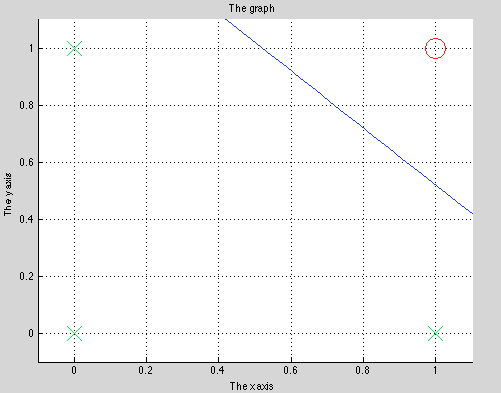
\includegraphics[scale=0.5]{learnConjunctions}\\
                (If you squint you can see the green x's at (0,0),(1,0),(0,1))\\
                For hw1conjunctions.txt, my returned values were (with some loss of precision so they could fit on the screen):
                    $$w = [2.910,
                          -2.049,
                           0.177,
                           190.519,
                           0.139,\\
                          -3.101,
                          -2.953,
                          -193.277,
                           1.167,
                          -8.894]^T$$
                    $$\theta = -90.2115$$
                    $$\delta = -2.4158e-13 \approx 0$$
               From this data, it's easy to guess what the target conjunction really is, since $w_4$ has such a huge weight, and $w_8$ has such a huge negative weight, the function must be $x_4 \land \neg x_8$, while the remaining values of $w$ can just be treated as negligible noise. Upon a cursory glance through hwconjunction1.txt, my prediction for the target conjunction looks correct. Geometrically speaking, this could be thought of in terms of the normal vector of a hyperplane. The large components will ``pull'' the normal of the plane in such a way that the hyperplane is almost perpendicular to the axis of that component, creating more separation on that component. The threshold, $\theta$, will affect the translation of our hyperplane in such a way that it actually separates the data. And $\delta$ is rightfully $0$.\\
        \item[b.3.] Learning Badges\\\\
                For the values after running learnBadges, I got $\delta = 1.2612e-09$, accuracyInTrain=$1$, accuracyInTest=$1$, and the following figure:\\
                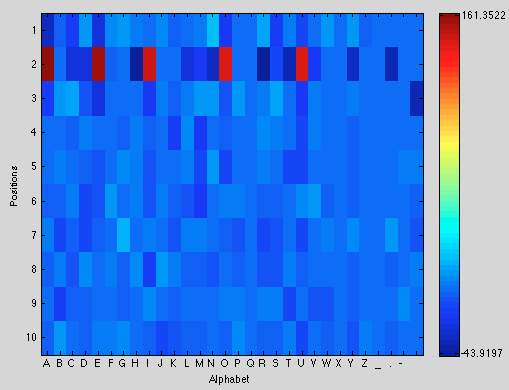
\includegraphics[scale=0.5]{learnBadges}\\
                It's clear to see that the function to check whether or not it's a positive example sees the 2nd position, and if it's a, e, i, o, or u, (a vowel), it marks it as positive. Rightfully so, the $\delta$ is approximately $0$, and the accuracy indicates 100\% on the test data.\\\\
                For my changed features, I changed positions from $[1,2,..,10]^T$, to $[1,3,5,7,9]^T$. (In matlab from 1:10 to 1:2:10). This resulted in an interested outcome of $\delta = 9.5511e-11$, as usual, accuracyInTrain=$1$, and accuracyInTest=$0.8298$. The figure generated was:\\
                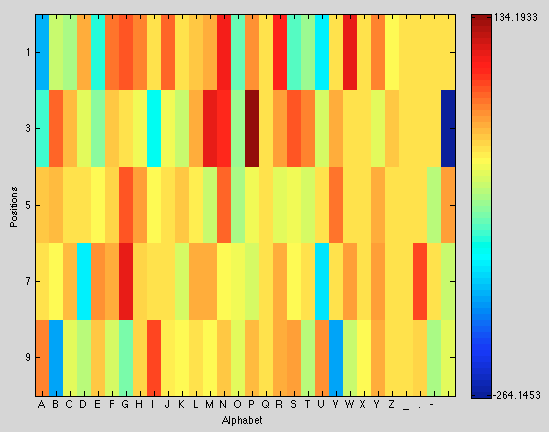
\includegraphics[scale=0.5]{learnBadges2}\\
                For the most part, it looks MUCH noisier than our last figure, but there is some sort of structure. For example, in the position of the first character, the vowels are pretty cool (negative weightage) perhaps because there are so few names that start out with two vowels in a row. Even if the actual important feature (2nd position) was ommited, it's not independent of the other positions, so my new feature set still does capture a great deal of information. If the characters of all the positions besides the 2nd were randomly distributed, this would not be the case, and we'd have nothing to learn from after ommitting the 2nd position from our feature set. (Just a disclaimer, when I say 2nd position, I mean the 2nd position for a,b,...,z.) I believe this is the reason the new features could still get a pretty good percentage of accuracy for the test data (82.98\%).
        \item[b.4.] Learning Multiple Hyperplanes\\\\
                 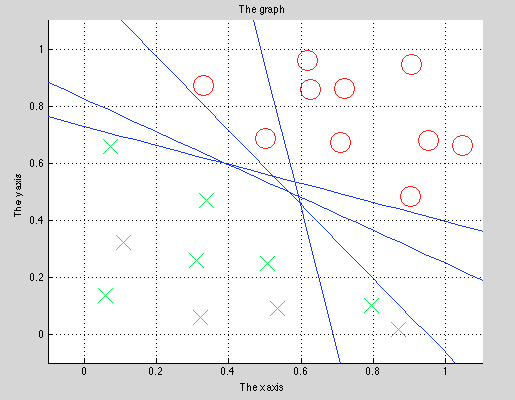
\includegraphics[scale=0.5]{learnMultipleHyperplanes}\\
                 All but the 4th hyperplane (as in the last one rendered in the Matlab file, where $w=[500,100]^T$) properly separated the data. As expected, the $\delta$ of the last hyperplane was $92.9650$, while all the others were approximately $0$. This reveals that there is a range that $w$ can be, or a certain margin of rotational ``wiggle room'' of the hyperplane for the data to still be linearly separable. By forcing $w$ to take on a very poor value, there was no solution that separated the data, and, accordingly, $\delta$ took on a large value. \\\\
                 If I were to pick, I'd pick the first hyperplane, with the $w$ value obtained from the solution of the original LP, rather than those other ones with imposed $w$s. Just visually, it seems to have the largest margin of distance between the positive and negative points, and I believe this would make it more robust for new sets of data to test on. The other (successful) hyperplanes get too close to the points, and have a very small margin, and would likely misclassify very close points when tested on real data.\\\\
                 Since we have multiple hyperplanes with $\delta \approx 0$, it's evident that the solution to the LP is not unique. The constraints are all the same, yet multiple values of $w$ and $\theta$ still result in a $\delta \approx 0$. This is all assuming that the difference between $-5.4570e-11$ and $-6.8212e-13$, for example, as reported by Matlab, are not different, both signifying $0$, and are just a result of floating point imprecision.\\\\\\
                
      \end{enumerate}
\item Code Snippets
      \begin{enumerate}
      \item [b.1.]
      \begin{verbatim}
function [w,theta,delta] = findLinearDiscriminant(data)
[m, np1] = size(data);
n = np1-1;

for i=1:m,
    if data(i,n+1) == -1
        data(i,:) = horzcat(data(i,1:n)*-1, data(i,n+1));
    end
end

A = vertcat( horzcat(data,ones(m,1)) , zeros(1,n+2) ); A(m+1 ,n+2)=1;
b = ones(m+1,1); b(m+1) = 0;
c = zeros(n+2,1); c(n+2) = 1;

[t, z] = linprog(c, -A, -b);

w = t(1:n);
theta = t(n+1);
delta = t(n+2);

end
      \end{verbatim}
      \item [b.2.]
      \begin{verbatim}
function plot2dSeparator(w, theta)
    x = linspace(-2,2,100);
    y = (-theta-w(1)*x)/w(2);
    plot(x,y);
end
      \end{verbatim}  
      \item [b.3.]
      \begin{verbatim}
function y = computeLabel(x, w, theta)
    thresh = dot(x,w)+theta;
    if(thresh >= 0)
        y=1;
    else
        y=-1;
    end
end
      \end{verbatim}
      \item [b.4.]
      \begin{verbatim}
function [theta,delta] = findLinearThreshold(data,w)
[m, np1] = size(data);
n = np1-1;

A = zeros(m,2);
b = zeros(m,1);
c = [0,1];

for i=1:m,
    if data(i,n+1) == -1
        A(i,:) = [-1,1];
        b(i,:) = 1 + dot(w,data(i,1:n));
    elseif data(i,n+1) == 1
        A(i,:) = [1,1];
        b(i,:) = 1 - dot(w,data(i,1:n));
    end         
end

A = vertcat(A, [0,1]);
b = vertcat(b, 0);

[t, z] = linprog(c, -A, -b);

theta = t(1);
delta = t(2);

end
      \end{verbatim} 
      \end{enumerate}
\end{enumerate}

\end{document}

